\chapter{\ifproject%
\ifenglish Project Structure and Methodology\else โครงสร้างและขั้นตอนการทำงาน\fi
\else%
\ifenglish Project Structure\else โครงสร้างของโครงงาน\fi
\fi
}

ในบทนี้จะกล่าวถึงหลักการ และการออกแบบระบบ

\makeatletter

% \renewcommand\section{\@startsection {section}{1}{\z@}%
%                                    {13.5ex \@plus -1ex \@minus -.2ex}%
%                                    {2.3ex \@plus.2ex}%
%                                    {\normalfont\large\bfseries}}

\makeatother
%\vspace{2ex}
% \titleformat{\section}{\normalfont\bfseries}{\thesection}{1em}{}
% \titlespacing*{\section}{0pt}{10ex}{0pt}

\section{เตรียมชุดข้อมูลฝึกสอน}
ข้อมูลที่ใช้ในการ train mode โดยมีสินค้าประมาณ 100 ชนิด โดยจัดเก็บข้อมูลใช้กล้องมือถือ ในการถ่ายภาพในมุมต่างๆ
ของสินค้าชนิดนั้นๆ ตามมุมต่างๆ จำนวนชนิดละ N รูป โดยจัดเก็บใน  และทำการดึงข้อมูลมา train ผ่าน Google Colab
 โดยโครงสร้างการเก็บข้อมูลจะเป็นดังรูป


 
\begin{center}
  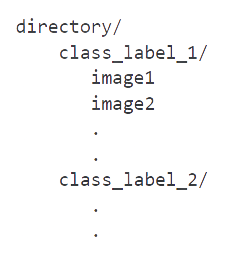
\includegraphics[scale=0.45]{pic/st.png}
\end{center}
  โดย
 
 
  
\subsection{Model Architecture}
โดยโมเดลในโครงงานนี้จะใช้ Xception pre-trained มาใช้ในการแยกคุณลักษณะของข้อมูล  และสร้างโมเดลมาต่อท้ายเพื่อ เรียนรู้จากข้อมูลที่ Xception แยกออกมาได้
\begin{center}
  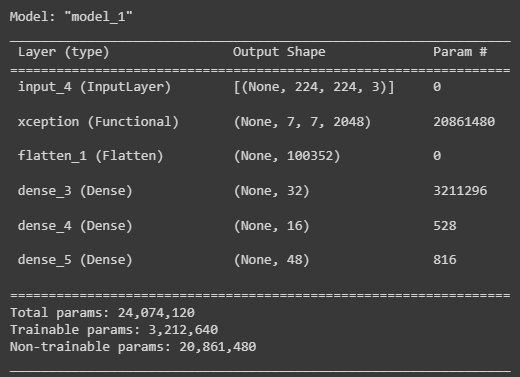
\includegraphics[scale=0.45]{pic/model.png}
\end{center}
  
นำมาต่อด้วย classifier ซึ่งเป็น Dense Layers สำหรับการ classify ชนิดของ products จากชุดข้อมูล

% \section{Product database}
% Section 2 text.

 

 
% \subsection{Transfer Learning}

Subsection 1 text

\section{classification products}

\begin{figure}[h]
  \begin{center}
  % 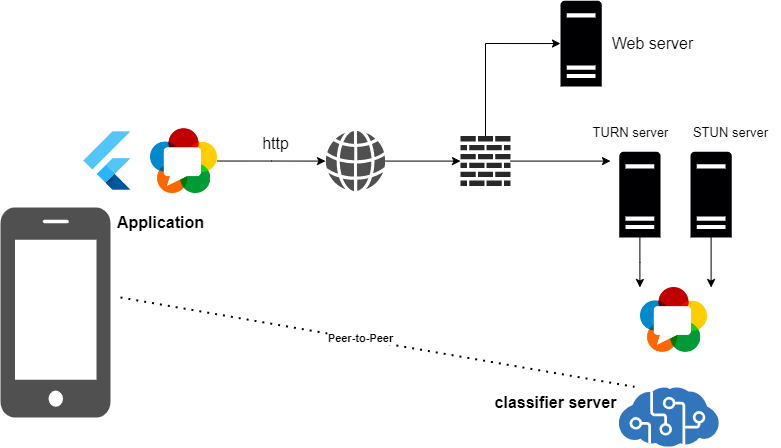
\includegraphics{pic/webrtc.png}
  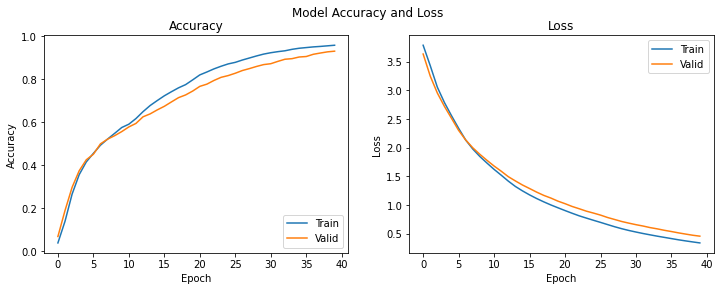
\includegraphics[scale=0.45]{pic/train.png}
  \end{center}
  
  \caption[Train results]{Train results}
  \label{fig:Train results}
  \end{figure}

% \begin{figure}[h]
% \begin{center}
% % 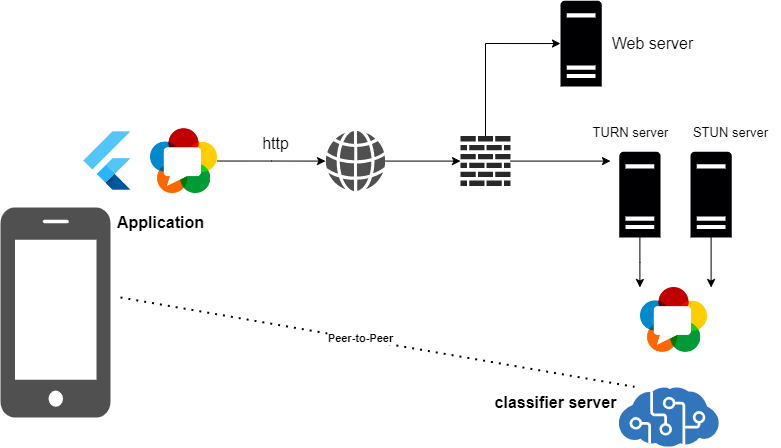
\includegraphics{pic/webrtc.png}
% 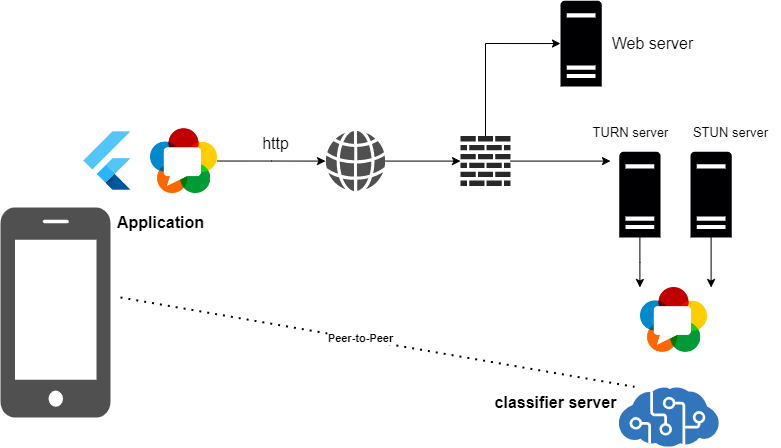
\includegraphics[scale=0.5]{pic/webrtc.png}
% \end{center}

% \caption[webrtc structure]{webrtc structure}
% \label{fig:webrtc structure}
% \end{figure}
\newpage

\section{การพัฒนา application }


\section{Product database }

\section{การพัฒนาweb dashboard }

ออกแบบ UI/UX ของเว็บไซต์และ application ด้วย Figma
ในส่วน application จะ  ใช้งาน Flutter และภาษา Dart และใช้ module  WebRTC ในการติดต่อกับ classifier ของ Backend

เพื่อ  sending a video feed from a flutter app to a python backend

 
\section{แผนภาพกระแสข้อมูล (Data Flow Diagram)}
\begin{figure}[h]
  \begin{center}
  % 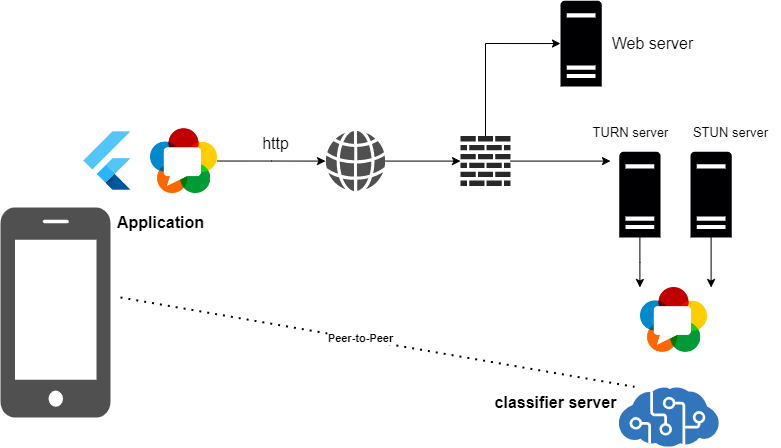
\includegraphics{pic/webrtc.png}
  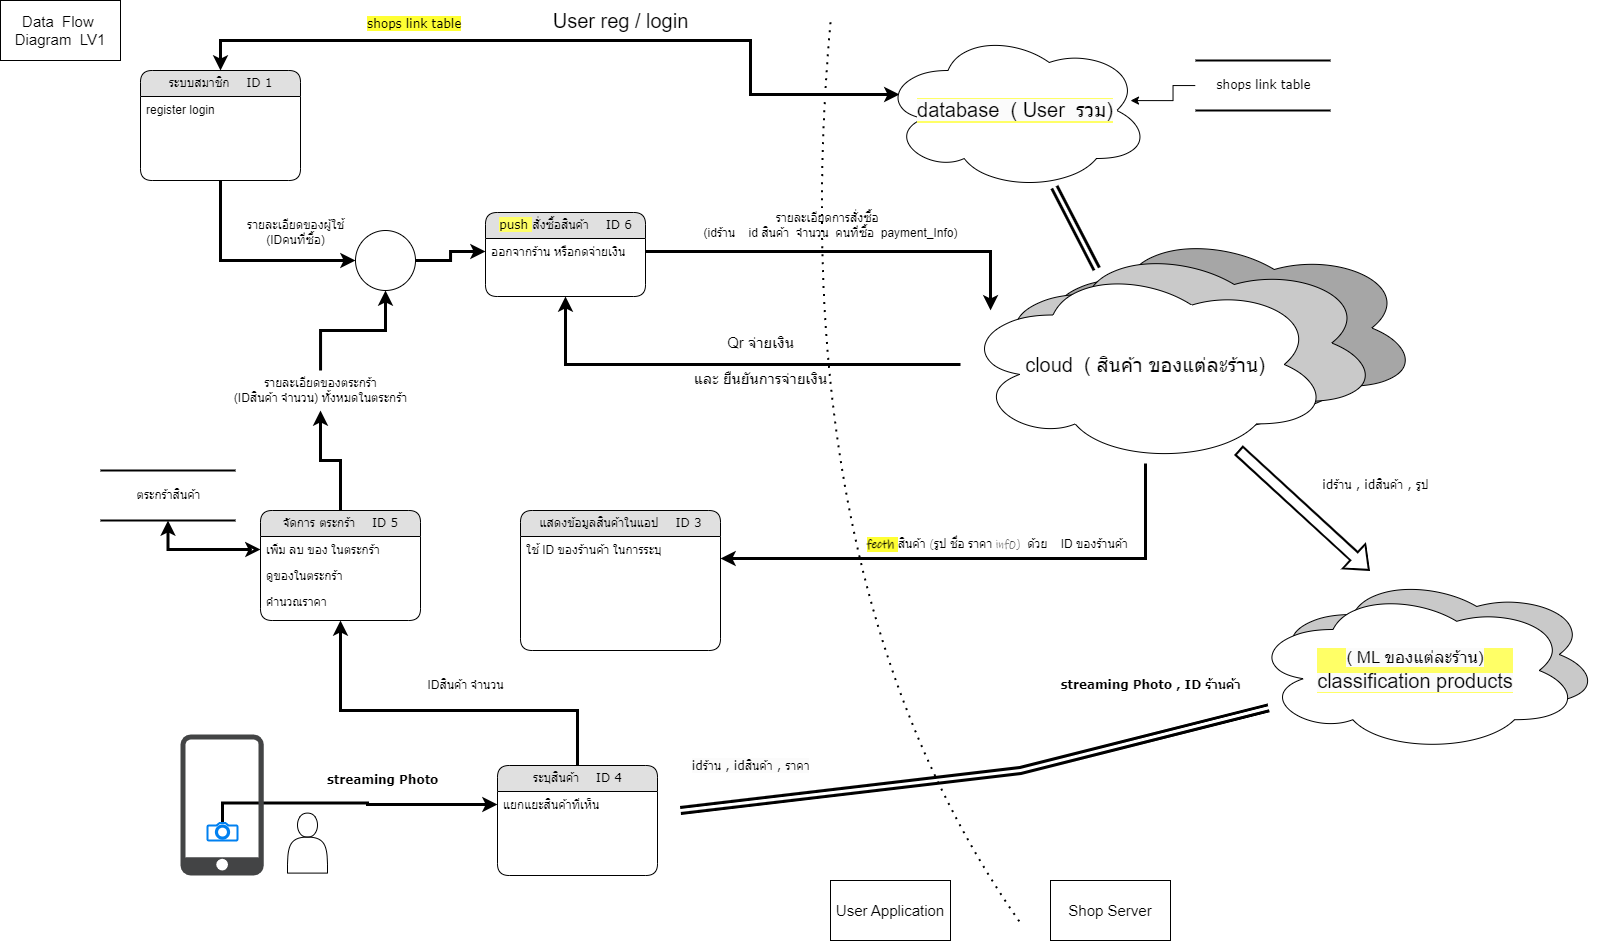
\includegraphics[scale=0.25]{pic/dataflow-lv0.png}
  \end{center}
  
  \caption[Data Flow Diagram]{Data Flow Diagram}
  \label{fig:Data Flow Diagram}
  \end{figure}
  

% \subsection{The Black Kitten}
  % One thing was certain, that the WHITE kitten had had nothing to
% do with it:---it was the black kitten's fault entirely



% ~\cite{aiw}. 




%  For the
% white kitten had been having its face washed by the old cat for
% the last quarter of an hour (and bearing it pretty well,
% considering); so you see that it COULDN'T have had any hand in
% the mischief.

%   The way Dinah washed her children's faces was this:  first she
% held the poor thing down by its ear with one paw, and then with
% the other paw she rubbed its face all over, the wrong way,
% beginning at the nose:  and just now, as I said, she was hard at
% work on the white kitten, which was lying quite still and trying
% to purr---no doubt feeling that it was all meant for its good.

%   But the black kitten had been finished with earlier in the
% afternoon, and so, while Alice was sitting curled up in a corner
% of the great arm-chair, half talking to herself and half asleep,
% the kitten had been having a grand game of romps with the ball of
% worsted Alice had been trying to wind up, and had been rolling it
% up and down till it had all come undone again; and there it was,
% spread over the hearth-rug, all knots and tangles, with the
% kitten running after its own tail in the middle.

% \subsection{The Reproach}

  